\documentclass[12pt,a4paper]{article}

\usepackage{fullpage}
\usepackage[utf8]{inputenc}
\usepackage{amsfonts}
\usepackage{amssymb}
\usepackage[french]{babel}
\usepackage[cyr]{aeguill}
\usepackage{natbib}
\usepackage{graphicx}
\usepackage{tabularx}
\usepackage{hyperref}
\usepackage[document]{ragged2e}
\setlength{\parindent}{2em}
\setlength{\parskip}{1em}

\newcommand{\quotes}[1]{``#1''}

\begin{document}

    \begin{titlepage}
        \centering
        {\scshape\LARGE Université de Bordeaux \par}
        {\scshape\Large Master 1 Informatique  \par}
        \vspace{3cm}

        {\Huge\bfseries Projet de Programmation\par}
        {\Huge\bfseries Le Clicodrome de LEFFF \par}
        {\Large\bfseries par Lionel CLEMENT \par}
        \vspace{0.5cm}
        {\Large\itshape Mémoire \par}
        {\large 4 Avril 2019\par}

        \vfill
        réalisé par \par
        BAKIR \textsc{Fatima Ezzahra} \par
        JELLITE \textsc{Oumayma} \par
        NEDELEC \textsc{Guillaume} \par
        SYLLA  \textsc{Alfred Aboubacar} \par
        \vfill

        {\large Enseignants responsables : Philippe NARBEL et Vincent PENELLE\par}

    \end{titlepage}

    \newpage
    \tableofcontents
    \newpage
    \listoffigures

    \newpage

    \section{Introduction}

    \subsection{Contexte}

    \smallbreak Lionel Clément est un enseignant-chercheur du Labri (Laboratoire Bordelais de Recherche en Informatique) informatique, spécialisé dans le domaine de la linguistique formelle et du traitement automatiques des langues. Il a réalisé avec Benoît Sagot, chercheur dans le même domaine à l'INRIA (Institut National de Recherche en Informatique et en Automatique), le Lexique des formes fléchies du français, appelé le LeFFF.

    Avant de détailler l’objectif de notre projet, nous allons mettre
    au clair quelques notions nécessaires à la compréhension du sujet.
    On appelle "lemme" un mot qui, de quelque nature que ce soit, qu'il soit composé ou simple, peut être référencé dans un dictionnaire.
    Dans la langue française, les formes fléchies correspondent aux conjugaisons et aux déclinaisons (forme au pluriel, forme féminine etc...) d'un lemme. Chaque forme fléchie est rattaché à un lemme particulier.
    Par exemple, "mangeront", "mange" et "mangera" sont trois formes fléchies du lemme "manger".

    Le LeFFF contient un grand nombre de mots de différentes catégories (noms propres, des noms communs, des adverbes, des adjectifs, etc...).
    Lionel Clément le qualifie comme "une ressource complexe constituée de
    \begin{itemize}
        \item Lexème ou grammème (ie Prendre)
        \item Vocables (ie Prendre=saisir, Prendre=recevoir)
        \item Catégories syntaxiques (ie Verbe)
        \item Sous-catégories syntaxiques (ie Transitif, passivable)
        \item Catégories grammaticales (ie Nombre$\rightarrow\{sing, plur\}$, Personne$\rightarrow\{1, 2, 3\}$)
        \item Règles de flexion (ie Table de conjugaison de prendre - Stem=.*(pren|mett))
        \item Valence (ie objet nominal, oblique en à)
        \item Réalisation syntaxique (ie passif en par)
        \item Phraséologie (ie "Prendre ombrage", "Prendre ses jambes à son cou")
        \item Collocation (ie "Prendre une initiative")
        \item Fonctions lexicales (ie Magn: "Prendre une belle initiative")
    \end{itemize}

    \smallbreak Aujourd'hui ce lexique est présent dans un fichier texte et il n'existe pas d'outils permettant de faciliter son accès, sa modification ou son enrichissement.
    Le système actuel n'assure pas une bonne traçabilité des modifications effectués par les linguistes et ne permet aucun contrôle de ces changements.

    L'objectif de ce projet est donc de transformer le lexique au format texte en une base de données et de développer une interface web, facilitant les interactions avec le lexique via cette base de données.
    L'avantage de cette solution web est que l'on ne sauvegarde dans la base de données, que les lemmes présents dans le lexique. On n'enregistre pas les formes fléchies afin de réduire considérablement la taille de la base.
    Les formes fléchies seront ensuite générées automatiquement par notre application à l'aide de règles, qui elles, seront enregistrées dans la base de données.
    Ces règles respectent le formalisme PFM (Paradigm Function Morphology) qui permet d'associer une forme flexionnelle à un lemme, passé en entrée avec ses propriétés morphosyntaxiques.

    Le projet peut être donc séparé en trois parties principales :
    \begin{itemize}
        \item L'importation du lexique dans une base de données
        \item La création de l'interface web qui interagira avec la base de données
        \item Le développement d'un interpréteur permettant de générer les formes fléchies d'un lemme donné en entrée selon des règles enregistrées en base de données.
    \end{itemize}

    \subsection{Description de l'existant}
    \subsubsection{Le lexique : LeFFF}
    Pour ce projet, nous avons a notre disposition différentes versions du Lefff dont la dernière version été réalisée par Benoît Sagot en 2010. Cette version est disponible dans 2 formats, à savoir \cite{lefff_int} :
    \begin{itemize}
        \item le lexique \textbf{intentionnel}, qui décrit pour chaque entrée, son lemme (forme canonique + tableau d'inflexion) ainsi que des informations syntaxiques profondes (cadre de sous-catégorisation profonde + réalisations possibles + restructurations possibles) .
        \item le lexique \textbf{extensionnel}, construit automatiquement par compilation du lexique intentionnel.
    \end{itemize}

    \smallbreak
    Le lexique extensionnel est présenté sous la forme ci-dessous :
    \begin{verbatim}
        démariés	adj	démarier	Kmp
        démariés	v	démarier	Kmp
        démarqua	v	démarquer	J3s
        démarquage	nc	démarquage	ms
        démarquages	nc	démarquage	mp
    \end{verbatim}

    \smallbreak La première colonne correspond à un mot du lexique.
    \smallbreak La seconde colonne présente la catégorie (\textbf{adj}(adjectif), \textbf{v}(verbe), \textbf{np}(nom propre), \textbf{nc} (nom commun) ) du mot.
    \smallbreak La troisième colonne présente le lemme auquel le mot est rattaché.
    On peut détecter si un mot est une forme fléchie d'un lemme si le contenu de la troisième colonne est différents de celui de la première.
    \smallbreak La dernière colonne apporte des informations sur le mot par le biais de tags. Ces informations peuvent être
    le genre, le nombre ou encore le temps utilisé pour conjuguer un verbe.
    Une explication de ces codes est disponible sur le site de Lionel Clément \cite{tagset}.

    Il existe un format extensionnel plus enrichi en tags que celui présenté ci-dessus. Vous le trouverez sur le site de Lionel Clément (version 2.1) ou de Benoît Sagot (format .elex).

    Le format intentionnel contient plus d'informations puisqu'il contient les paramètres morphologiques des mots.
    Néanmoins, nous ne le détaillerons pas plus car il ne sera pas pris en charge par notre application.

    \subsubsection{Le formalisme PFM}

    D'après la documentation \cite{Formalisme} de Olivier Bonami et Gilles Boyé, le formalisme Paradigm Function Morphology est présenté comme une théorie explicite de la morphologie flexionnelle qui est à la fois inférentielle (qui présente une conclusion à partir d'un fait, d'une situation) et réalisable. Les affixes ne sont pas traités comme des signes, mais comme des résultats de l'application d'une règle liant les caractéristiques morphosyntaxiques à une fonction phonologique qui modifie une base.
    Dans le formalisme PFM, le système flexionnel d'un langage est modélisé par une fonction de paradigme.
    Les fonctions de paradigme prennent en entrée une racine et un ensemble de fonctions, et retournent un ensemble phonologique.

    La forme générique des fonctions paragigmes est : \textbf{PF(l, $\sigma$) = IV o III o II o I (l,$\sigma$)($\epsilon$)}
    \begin{itemize}
        \item l : lemme auquel on souhaite appliquer le formalisme
        \item $\sigma$ : série de tags que l'on souhaite appliquer au lemme
        \item IV o III o II o I : Niveaux d'applications des règles
    \end{itemize}

    \smallbreak

    De manière plus formelle, le formalisme indique que pour un lemme donné avec une série de tags, une règle de chaque niveau d'application (et une seule uniquement pour chaque niveau), correspondant aux tags renseignés, va être appliqué au lemme. \\
    Si pour un niveau d'application, aucune règle ne correspond, le formalisme passe au niveau d'application suivant. \\
    Si pour un niveau d'application, plusieurs règles correspondent, celle qui s"applique sera celle qui comporte le plus de tags (la règle la plus spécifique).

    \smallbreak
    Le format de base des règles est de la forme : \textbf{n, X, t $\Longrightarrow$ f(X) } \\
    \begin{itemize}
        \item n : niveau d’application de la règle
        \item X : lemme
        \item t : combinaison de tags pour laquelle la règle s'applique (Tous les tags doivent être renseigné par l'appel du formalisme pour que la règle puisse s'appliquer
        \item f(X) : la forme flexionnelle
    \end{itemize}

    Prenons un exemple concret du formalisme PFM avec les règles suivantes : \\
    \begin{itemize}
        \item I, chaîne,{f} $\Longrightarrow$ chaîne + "ne"
        \item II, chaîne, {p} $\Longrightarrow$ chaîne + "s"
    \end{itemize}

    On applique le formalisme sur le lemme "Sien" et lui appliquer le féminin et le pluriel : \\
    PF(Sien, {f,p} ) = IV o III o II o I (Sien, {f,p} )(\textbf{$\epsilon$}) \textit{Application de la règle I} \\
    = IV o III o II (Sien, {f,p} )(\textbf{Sienne}) \textit{Application de la règle II} \\
    = IV o III (Sien, {f,p} )(\textbf{Siennes}) \textit{Aucune règle à appliquer} \\
    = IV (Sien, {f,p} )(\textbf{Siennes}) \textit{Aucune règle à appliquer} \\
    =\textbf{ Siennes }

    Dans cet exemple, on souhaite appliquer le féminin et le pluriel au lemme "Sien".
    La syntaxe montre l'application des règles de niveau 1 avant l'application des règles de niveau 2.
    Cette hiérarchie des niveaux d'application est nécessaire pour éviter toute incohérence. Ce système garantie que le résultat sera "Siennes". Il sera donc impossible d'obtenir "Siensne". \\
    D'autres exemples sont disponible dans la documentation de Olivier Bonami \cite{PFM}.

    \newpage
    \section{Analyse des besoins}

    Afin d'avoir une vision globale sur le projet, nous avons fais une analyse pour hiérarchiser les besoins du client.
    Nous avons décrit les besoins fonctionnels (fonctionnalités de l'application) et les besoins non fonctionnels (qualité logicielle, sécurité etc...).

    \subsection{Analyse des besoins fonctionnels}

    Pour apporter un contrôle des interactions des utilisateurs depuis le site web, un système de rôle doit être mis en place. Avant de présenter la liste des besoins fonctionnels identifiés, voici une présentation de ces différents rôles utilisateurs, qui vous aidera a mieux comprendre ces besoins :
    \begin{itemize}
        \item \textbf{Les visiteurs} : Ils ne peuvent que rechercher, consulter les mots du lexique, signaler des erreurs sur un mot ou exporter le lexique.
        \item \textbf{Les éditeurs} : Ce type d'utilisateur peut, en plus d'avoir les mêmes droits que les visiteurs, modifier un mot (ou ses attributs) du lexique. Ces actions ne peuvent être effectuées qu'en étant connecté (via un système d'authentification) sur le site.
        \item \textbf{Les éditeurs experts} : Ces utilisateurs sont des éditeurs pouvant supprimer définitivement des mots du lexique. Ces utilisateurs peuvent aussi ajouter/modifier/ supprimer des catégories et des règles PFM.
        \item \textbf{Les administrateurs} : Ils ont un contrôle total de l'application. En plus d'agir comme des éditeurs expert, ce sont eux qui gèrent les différents utilisateurs du site (validation d'inscription, bannissement d'utilisateurs ou changement de rôle).
    \end{itemize}

    \smallbreak

    \begin{figure}[h]
        \centering
        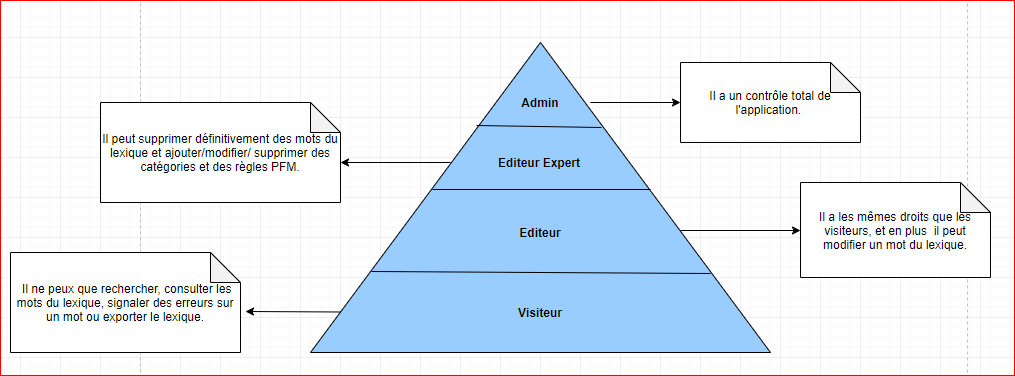
\includegraphics[width=150mm]{img/role.PNG}
        \caption{Gestion des rôles}
        \label{Tux}
    \end{figure}

    La liste des besoins présentée ci-dessous a été triée par domaine d'action. Les priorités de chaque besoin vont de la priorité 1 (la plus prioritaire) à la priorité 3 (la moins prioritaire).

    \subsubsection{Gestion du lexique LeFFF}

    \textbf{Création d'une base de donnée} \\
    \textbf{Priorité : 1} \\
    Il est nécessaire de créer la base de données ainsi que les tables et les relations entre les tables pour qu'elle soit prête à enregistrer les informations du lexique, nécessaires au bon fonctionnement de l'application.

    \textbf{Importer le LeFFF dans la base de données} \\
    \textbf{Priorité : 1} \\
    Pour ce besoin, nous devons analyser le lexique qui nous est fourni (au format .txt ou .mlex) et en extraire les lemmes et leurs informations (tags, catégories...) afin de les enregistrer dans notre base de données préalablement configurée.
    Cette fonctionnalité est nécessaire pour filtrer le nombre d'entrée à enregistrer sur le grand nombre proposé par le lexique (environ 100 000 entrées à enregistrer sur les 500 000 entrées du lexique, dans le leFFF en version 2.1).

    \textbf{Exporter le Lefff} \\
    \textbf{Priorité : 3}  \\
    Tous les utilisateurs peuvent effectuer une exportation du lexique.
    Cette fonctionnalité sera disponible depuis notre application web et nécessitera l'utilisation d'un interpréteur PFM pour générer les formes fléchies des mots présents dans la base de données.

    \subsubsection{Manipulation du lexique}

    \textbf{Rechercher un mot} \\
    \textbf{Priorité : 2} \\
    Un champ de recherche, disponible pour tous les utilisateurs, permet de rechercher un mot du lexique. A la manière d'un moteur de recherche classique, la liste des mots enregistrés dans notre base de données, correspondant à ce qui a été recherché apparaîtront sur la page. Il sera ensuite possible à l'utilisateur de consulter en détail un mot, de signaler une erreur, de le modifier ou le supprimer (Si les droits de l'utilisateur le lui permet). Si aucun mot ne correspond en base de données, un message d'avertissement apparaîtra sur l'interface.

    \textbf{Consulter un mot} \\
    \textbf{Priorité : 2} \\
    Disponible après avoir effectué une recherche, la consultation d'un mot permet d'obtenir un écran détaillant les caractéristiques du mot (catégorie, tags...) ainsi que toutes les formes fléchies générées pour ce mot.
    Si les droits de l'utilisateur le permet, les boutons d'ajout, de modification et de suppression apparaissent également sur cet écran.

    \textbf{Ajouter un mot} \\
    \textbf{Priorité : 2} \\
    Cette partie est réservée au utilisateurs authentifiés (les administrateurs, les éditeurs et les éditeurs experts).
    Un formulaire est proposé, où il est demandé de renseigner le mot à ajouter, sa catégorie (parmi celle enregistrées dans la base de données), et ses éventuels tags (saisie libre).
    Lors de l'ajout, des vérifications seront effectuées afin de vérifier si le mot n'existe pas déjà en base et que tous les champs renseignés ont des valeurs cohérentes.

    \textbf{Signaler un mot} \\
    \textbf{Priorité : 3} \\
    Les visiteurs et les éditeurs ont la possibilité de signaler des erreurs sur un mot.
    Ce mécanisme permet d'envoyer une notification aux administrateurs pour leur faire part d'informations sur un mot en particulier.
    En l'absence de la fonctionnalité de suppression ou de modification (pour les visiteurs), ce service permet à ces utilisateurs de faire remonter des erreurs ou des demandes particulières relatifs à des mots.

    \textbf{Modifier un mot} \\
    \textbf{Priorité : 2} \\
    En réutilisant le même formulaire que celui de l'ajout d'un mot, cette fonction de modification permet de modifier les informations d'un mot en pré-remplissant le formulaire avec les informations existantes. Elle est accessible à tous les utilisateurs connectés. Comme pour l'ajout, des vérifications seront effectuées à la soumission du formulaire (champs correctement remplis et doublons en base de données).

    \textbf{Supprimer un mot} \\
    \textbf{Priorité : 2} \\
    Les éditeurs experts et les administrateurs peuvent supprimer un mot de la base de données. Il leur suffit simplement de rechercher un mot et de sélectionner l'option "Supprimer". Un message de confirmation apparaîtra pour confirmer la demande de suppression avant de l'exécuter.

    \subsubsection{Génération des formes fléchies}
    \textbf{Priorité : 1} \\
    Ce besoin est le besoin principal de notre projet. En effet la génération dynamique des formes fléchies permet de réduire considérablement la taille du lexique à enregistrer dans la base de données.
    Pour répondre à ce besoin, il nous faut mettre en place un interpréteur permettant de traduire des règles PFM pour en générer des formes fléchies.

    \subsubsection{Gestion des règles}

    Les éditeurs experts et les administrateurs ont besoin de pouvoir gérer les règles PFM. En effet ces règles sont nécessaires à la génération des formes fléchies. Il faut donc proposer une interface permettant d'ajouter de nouvelles règles, les modifier ou encore les supprimer.

    \textbf{Ajouter / Modifier une règle}  \\
    \textbf{Priorité : 1} \\
    Ces écrans proposent un formulaire contenant les informations spécifique de la règle (niveau d'application, résultats ect...). dans le cas de la modification, les champs seront pré-remplis des informations existantes.
    Des vérifications seront effectués à la soumission du formulaires (validité des champs, gestion des doublons).

    \textbf{Supprimer une règle}  \\
    \textbf{Priorité : 1} \\
    Comme pour la suppression des mots, un message de confirmation apparaîtra pour confirmer la demande avant de l'exécuter.

    \subsubsection{Gestion des combinaisons de tags}

    Les règles PFM prennent des tags en paramètres pour détecter si elles doivent s'appliquer ou non.
    Les combinaisons de tags correspondent à des séries de tags appelé sur un mot pour génerer une forme fléchie.
    Les règles s'appliquent sur le mot si les tous ses tags (tags de la règle) sont reseignés dans les tags de la combinaison.

    \smallbreak

    Prenons un exemple simple avec des règles :
    \begin{itemize}
        \item I, root, \{a\} $\Longrightarrow$ root + RES1
        \item I, root, \{a,b,c\} $\Longrightarrow$ root + RES2
        \item III, root, \{b,c,d,e\} $\Longrightarrow$ RES3 + root
    \end{itemize}
    On appelle ensuite le formalisme PFM avec 3 combinaisons de tags (\{a\}, \{a,b,c,d\} et \{a,b,c,d,e\}) \\
    Nous obtenons les cas suivants :
    \begin{itemize}
        \item PF(myWord, \{a\}) = myWordRES1 \\
        Seul la première règle possède tous ces tags ("a") dans la combinaison renseignés. Seul cette règle s'appliquera.
        \item PF(myWord, \{a,b,c,d\}) = myWordRES2 \\
        Dans ce cas, les 2 premières règles correspondent (La troisième possède "e" qui n'est pas renseigné dans la combinaison). Or les 2 règles ont le même niveau d'application. On choisi donc la règle la plus spécifique (avec le plus de tags), soit la seconde.
        \item PF(myWord, \{a,b,c,d,e\}) = RES3myWordRES2 \\
        Toutes les règles correspondent, une sélection se fait entre les 2 premières règles comme dans le cas précédent.
    \end{itemize}

    \smallbreak

    Ces combinaisons sont donc nécessaires à la générations des formes fléchies. Si aucune combinaisons n'est renseignées alors aucune forme fléchie ne sera générée. Il y a une équivalence entre les formes fléchies et les combinaisons de tags : une combinaison de tags = une forme fléchie générée.
    \\
    Nous devons donc ajouter à notre interface, de quoi ajouter des combinaisons, modifier les combinaisons existantes et la possibilité de les supprimer. Ces fonctionnalités ne sont disponibles qu'aux éditeurs experts et aux administrateurs.

    \smallbreak

    \textbf{Ajouter / Modifier une combinaison}  \\
    \textbf{Priorité : 1} \\
    Mise en place d'un formulaire avec des vérifications de doublons en base de données à la soumission du formulaire.

    \textbf{Supprimer une combinaison} \\
    \textbf{Priorité : 1} \\
    Présence d'un message de confirmation de suppression avant d'exécuter la suppression.

    \subsubsection{Gestion des catégories}

    Les catégories permettent de classer les mots, les règles et les combinaisons de tags. En effet les règles qui s'appliqueront pour des verbes ne seront pas les mêmes que celles qui s'appliquent pour les noms communs.
    Il nous faut donc aussi fournir des interfaces permettant d'interagir avec les catégorie (disponible pour les éditeurs experts et les administrateurs).

    \textbf{Ajouter/Modifier une catégorie} \\
    \textbf{Priorité : 2 } \\
    Mise en place d'un formulaire avec des vérifications de doublons en base de données à la soumission du formulaire.

    \textbf{Supprimer une catégorie} \\
    \textbf{Priorité : 2 } \\
    Présence d'un message de confirmation de suppression avant d'exécuter la suppression.

    \subsubsection{Gestion des utilisateurs}
    Pour ajouter de nouveau utilisateurs et gérer les rôles de ceux existants, il est nécessaire de fournir une interface pour les administrateurs leurs permettant d'effectuer ces tâches.

    \textbf{Ajouter/Modifier un utilisateur} \\
    \textbf{Priorité : 3 } \\
    Mise en place d'un formulaire avec des vérifications de doublons en base de données à la soumission du formulaire.

    \textbf{Supprimer un utilisateur} \\
    \textbf{Priorité : 3 } \\
    Présence d'un message de confirmation de suppression avant d'exécuter la suppression.

    \subsubsection{Traçabilité des modifications}
    \textbf{Priorité : 3} \\
    Afin de garder une trace de tous les changements effectués, le besoin de sauvegarder ces changements permet de pouvoir revenir à un ancien état du lexique en faisant les changements inverses de ceux enregistrés.

    \subsection{Analyse des besoins non fonctionnels}

    \subsubsection{Généralisation de l'architecture}
    \textbf{Priorité : 1} \\
    Ce projet a été proposé spécifiquement pour le LeFFF. Néanmoins il est important de réaliser l'architecture de notre application web de la manière la plus générale possible.
    Le but étant que notre solution fonctionne correctement pour n'importe quel langage (en supposant que les données enregistrées dans la base soient cohérentes).

    \subsubsection{Alerter les utilisateurs}
    \textbf{Priorité : 2} \\
    Afin d'éviter un maximum les erreurs de manipulations, toutes actions entraînant la suppression d'éléments de la base de données seront précédées de l'affichage de message de confirmation afin d'alerter les utilisateurs de la suppression à venir.
    La mise en place de logs permettra de tracer les changements si une suppression a été effectuée par inadvertance.

    \subsubsection{Sécurité}
    \textbf{Priorité : 1} \\
    Afin de protéger l'intégrité des données du LeFFF dans la base de données, nous sécuriserons la base et l'application web des problèmes de sécurité suivants :
    \begin{itemize}
        \item \textbf{L'erreur humaine} : en cas d'oubli de déconnexion, la session de l'utilisateur peut être utilisée pour effectuer des changements non voulus. \\
        \textbf{Notre solution :} Un système de déconnexion automatique permet de répondre à ce problème en déconnectant l'utilisateur automatiquement après 10 minutes d'inactivité.

        \item \textbf{Les injections SQL}, permettant de récupérer ou d'altérer des données, voir même prendre le contrôle de serveur. L'attaque par injection SQL consiste à injecter du code malicieux SQL qui sera interprété par le moteur de base de données dans un champ de saisie d'une application web. \\
        \textbf{Notre solution :} Afin de se protéger de se genre d'attaque, nous avons choisi de développer l'application web en PHP avec le framework Symfony, qui comprend un l'ORM (Object-Relational Mapping) Doctrine. Cet ORM est une couche d'abstraction de base de données qui permet d'interagir avec le contenu de la base de données en manipulant des objets (informatique) du coté de notre application. Il comprend des modules de sécurité (génération de contraintes, formatage des données envoyées ect...) qui détecte les attaques par injection SQL.

        \item \textbf{Le Cross-Site Scripting (XSS)} : Cette faille permet d'injecter du code malicieux sur une page web. Par exemple sur un forum, si quelqu'un entre en commentaire un code Javascript nuisible, tous les autres utilisateurs qui accéderont à cette page seront impacté par ce code qui s'exécutera sur leur navigateur. \\
        \textbf{Notre solution :} Pour remédier à cela, le framework Symfony possède aussi un système (filtrage des données d'entrées, échappement des données en sortie...) protégeant de ce genre d'attaque afin de filtrer tous ce qui pourrait ressembler à du code. C'est un procédé assez similaire à celui de la protection contre les injections SQL.

        \item \textbf{La falsification de requête inter-sites (CSRF)} : Cette faille permet à un attaquant de forcer ses victimes à effectuer certaines actions sur un site cible, sans qu'elles s'en aperçoivent. Pour cela, les attaquants cherche à ce que leur victime visite une page (en étant connecté) où des scripts malicieux seront exécutes sans que la victime s'en aperçoive à l'aide de balise image chargeant le script par exemple. La victime étant authentifié sur le site, les scripts pourront s'exécuter correctement et corrompre les données du site. \\
        \textbf{Notre solution :} Voici la dernière faille de sécurité à laquelle Symfony nous protège. En effet le framework fait cela en générèrant des jetons ("tokens") au moment de l'authentification, différents pour chaque utilisateur et qui sont stockés dans la session. Ce jeton est ensuite vérifié a chaque action avec la base afin de vérifier que c'est bien une action voulue par l'utilisateur et non une attaque CSRF.
        \item \textbf{Le déchiffrement de données} qui consiste à déchiffrer des données crypté. Cela peut permettre de trouver des mot de passe et donc prendre le contrôle d'une session utilisateur ou bien de découvrir des informations sensibles (informations bancaire, personnelles...) \\
        \textbf{Notre solution :} Pour éviter cela, nous avons décidé de chiffrer les données avec des algorithmes irréversible (une fois crypté, aucune technique connue à ce jour peut décrypter le mot, il faut forcement connaître le mot initial) comme "bcrypt" ou "sha512".

        \item \textbf{L'écoute de communication réseau} : Requêter un site web avec un protocole HTTP permet à des intrus présent sur votre réseau de lire ou modifier le site internet que vous souhaitez consultez et présente donc un gros risque. \\
        \textbf{Notre solution} : Utiliser le protocole HTTPS qui permet de chiffrer les données échangées et ainsi les protéger de toutes interceptions ou modification.
    \end{itemize}

    \subsubsection{Format de fichier}
    \textbf{Priorité : 2} \\
    Afin de pouvoir répondre aux besoins d'importation et d'exportation du LeFFF avec la base de données, il nous faut définir les format de fichiers compatibles avec ces fonctions.
    Nous avons fait le choix d'utiliser les formats texte et mlex (.txt et .mlex)  car ce sont les formats disponibles au téléchargement du LeFFF actuellement. Ce choix nous permet de pouvoir exploiter le LeFFF existant sans avoir à le reformatter dans un format particulier.

    \subsubsection{Performances}
    \textbf{Priorité : 3} \\
    Au niveau des performances, le besoin se porte sur le temps de génération des formes fléchies. En effet l'algorithme de génération des formes fléchies doit être le plus optimisé possible pour réduire le temps d'exécution.
    Il en va de même pour l'importation du lexique et l'exportation.
    Ces performances doivent être optimales pour combler les temps d'exécution des requêtes SQL sur lesquelles nous n'avons pas de contrôle.

    \subsubsection{Ergonomie}
    \textbf{Priorité : 4} \\
    Un design très simple et épuré permet de faciliter l'utilisation de l'application par les utilisateurs. Cela leur permet de naviguer dans l'application de la manière la plus naturelle possible.
    \smallbreak
    Des codes couleurs et des icônes distinctifs permettent aussi de guider facilement l'utilisateur dans l'interface (ex: le rouge pour la suppression)

    \newpage
    \section{Architecture et implémentation de l'application web}

    \subsection{Architecture de la base de données }

    \begin{figure}[h]
        \centering
        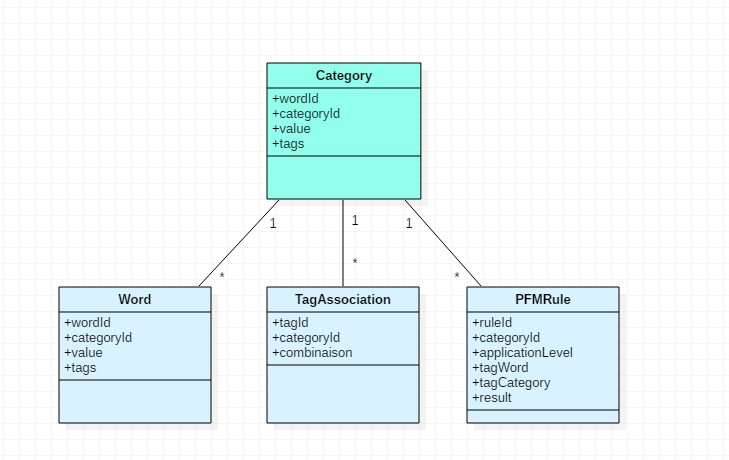
\includegraphics[width=150mm]{img/Capture.PNG}
        \caption{Architecture: Base de données}
        \label{Tux}
    \end{figure}

    Notre base de données est constituée de quatre tables :
    \begin{itemize}
        \item \textbf{Category} : Cette table contient le code et le nom de la catégorie.
        Le code est utilisé pour simplifier l'import du lexique puisque le LeFFF existant présente les catégorie avec des codes (par exemple : "adj" pour les adjectifs ou "v" pour les verbes).
        \item \textbf{Word} : Cette table est utilisé pour les mots du lexique. Elle y référence la valeur du mot, les tags qui peuvent lui être associé ainsi que l'identifiant de la catégorie auquel le mot appartient.
        \item \textbf{TagAssociation} : Cette table contient les combinaisons de tags utilisées pour générer les formes fléchies. Ces combinaisons sont liés à une unique catégorie via la clé étrangère "categoryId"
        \item \textbf{PFMRule} :Les règles PFM sont enregistrées dans cette table. \\
        Les règles sont liés à une unique catégorie par la clé étrangère "categoryId". \\
        Le résultat de la règle est enregistré grâce à l'attribut "result" (exemple de résultat ajoutant le suffixe "ent" à un mot : "\{word\}ent"). \\
        "applicationLevel" représente le niveau d'application de la règle. \\
        Enfin nous avons modifié le fonctionnement du formalisme PFM en dissociant les tags d'une règle en deux parties distinctes :
        \begin{itemize}
            \item "tagCategory" qui représente les tags de la règle que l'on va comparer avec les combinaisons de tags de la table "TagAssociation" pour savoir si la règle s'applique.

            \item "tagWord" qui représente des tags renseigné dans la table "Word". De la même façon que "tagCategory", si tous les tags d'un mot renseignés (dans la table "Word") sont présent dans l'attribut "tagWord" de la règle, alors la règle pourra potentiellement s'appliquer. Dans le cas contraire la règle est ignorée par l'interpréteur PFM.
        \end{itemize}
        Cette séparation nous permet par la suite d'optimiser les performances de l'algorithme de génération des formes fléchies dont le fonctionnement sera expliqué peu après.

    \end{itemize}
    \smallbreak
    Cette architecture de la base de données permet de généraliser notre application à n'importe quelle langage.
    Au lieu d'enregistrer des informations sous formes d'attributs dans la base de données, toutes les informations nécessaires à la génération des formes fléchies sont enregistrés sous forme de tags. Cela permet de ne pas restreindre l'utilisation de l'application à un langage spécifique.
    Le bon fonctionnement de l'application ne dépend ainsi que de la cohérence des données présentes dans la base de données.

    \subsection{Présentation de l'application web}

    \begin{figure}[h]
        \centering
        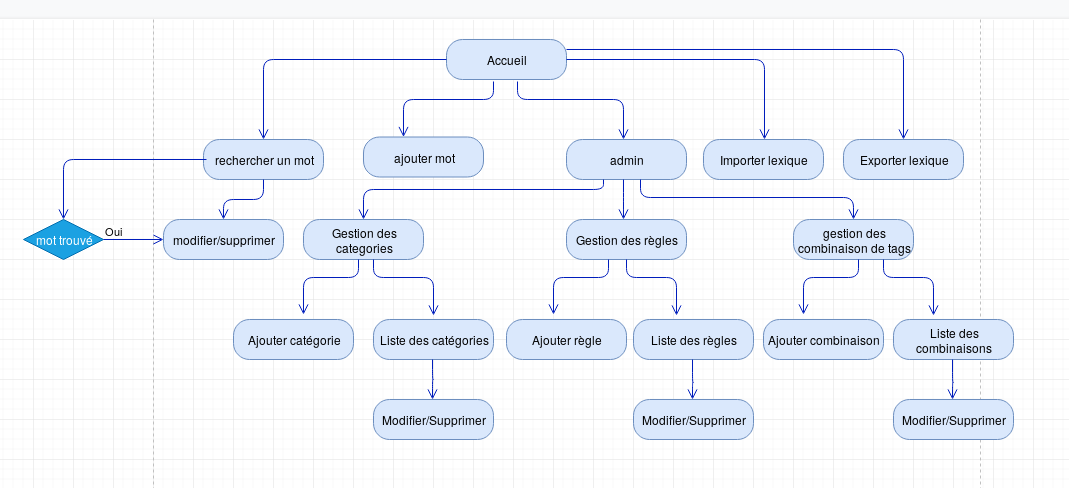
\includegraphics[width=150mm]{img/site1.png}
        \caption{Accessibilité des fonctionnalités sur l'application web}
        \label{Tux}
    \end{figure}

    Ce diagramme présente la navigation entre les différentes fonctionnalités de l'application web.

    \subsection{Présentation des interfaces}

    \textbf{ Rechercher Mot }

    Les utilisateurs peuvent consulter la liste des formes fléchies du mot comme il est montré dans la figure ci-dessus:

    \begin{figure}[h]
        \centering
        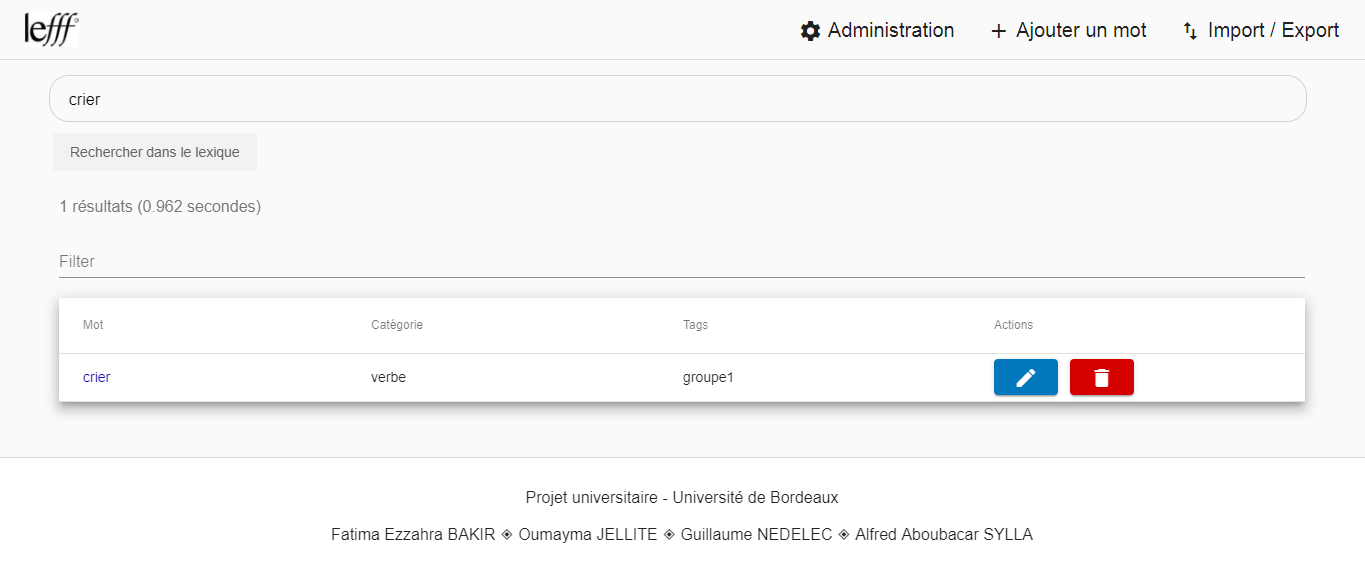
\includegraphics[width=150mm]{img/Recherche.PNG}
        \caption{Interface: Rechercher un mot}
        \label{Tux}
    \end{figure}

    L’utilisateur (l’administrateur) peut gérer le mort en le modifiant ou le supprimer.

    \textbf{ Ajouter mot}

    L'administrateur a le droit d'ajouter des nouveaux mots en accédant à l'interface suivante:

    \begin{figure}[h]
        \centering
        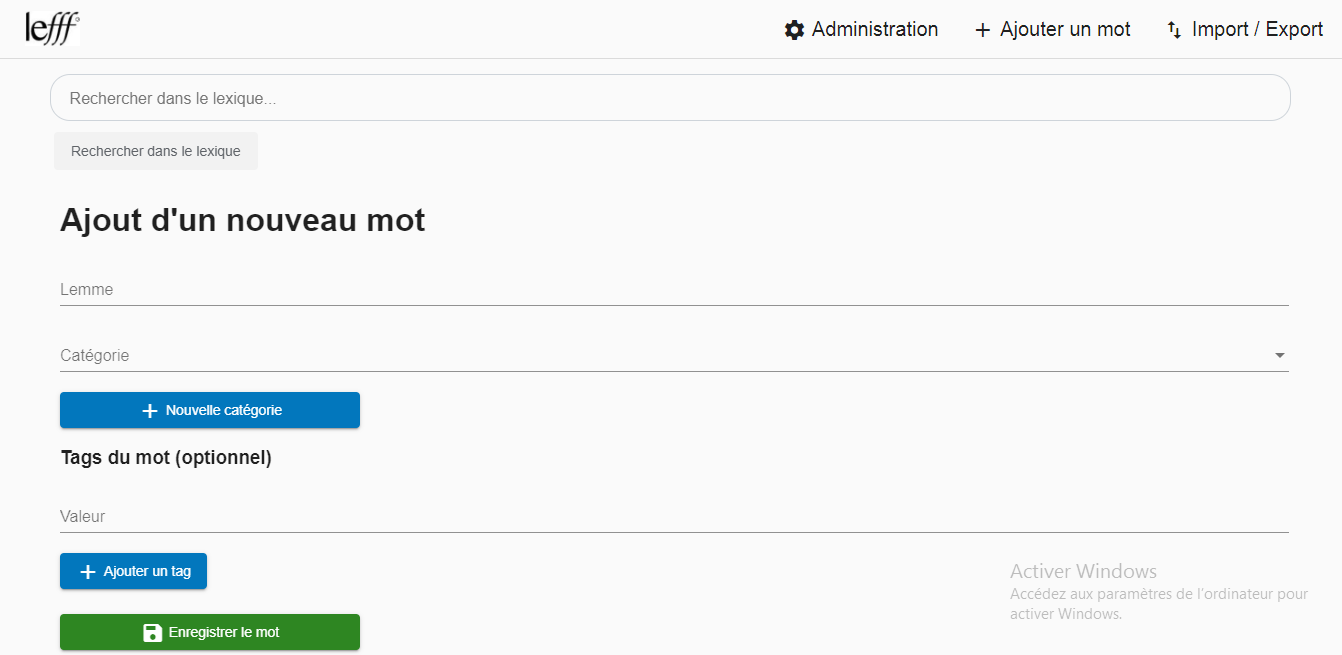
\includegraphics[width=150mm]{img/Ajoutermot.PNG}
        \caption{Interface: Ajouter un mot}
        \label{Tux}
    \end{figure}

    Si le mot est ajouté, un message d'information s'affiche. Une fois il est ajouté, l'utilisateur peut cliquer sur les boutons "Modifier" ou "Supprimer" si il a commis une erreur comme le montre la figure suivante:

    \textbf{Éditer un mot}
    \begin{figure}[h]
        \centering
        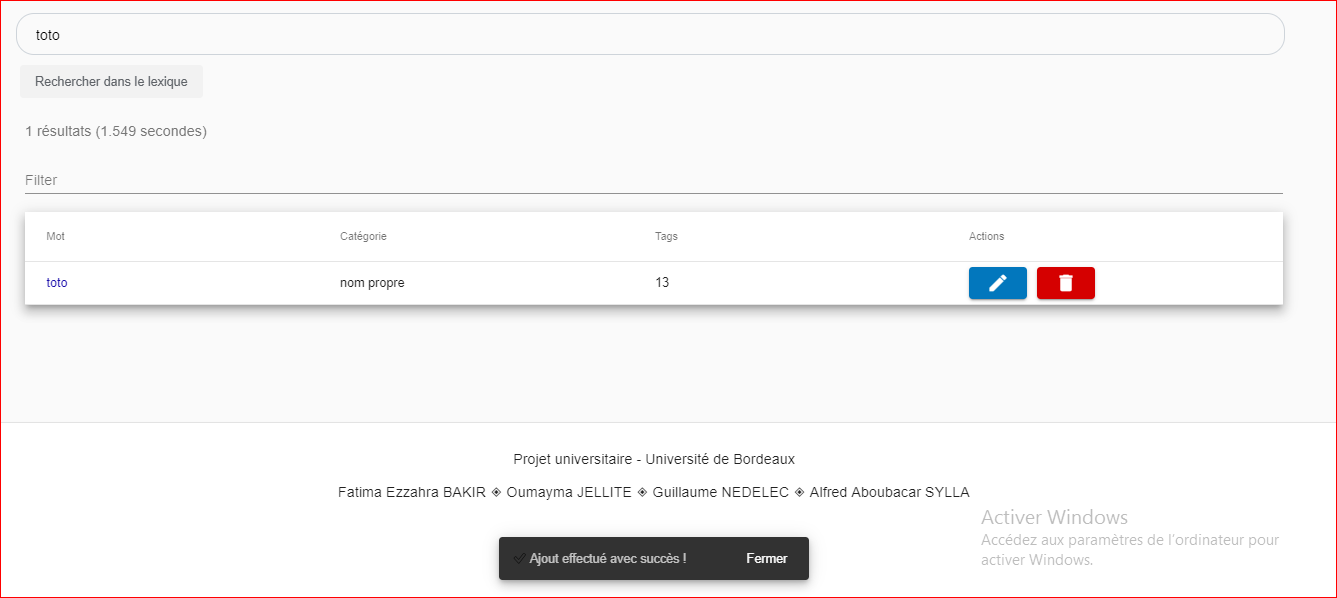
\includegraphics[width=150mm]{img/AjoutEffectuer.PNG}
        \caption{Interface: Éditer un mot}
        \label{Tux}
    \end{figure}

    comme il est montré sur la figure ci-dessus nous avons mis en place une interface pour pouvoir éditer un mot ; modifier ,supprimer et consulter un mot juste en cliquant sur les boutons présente sur l'interface .
    Nous avons fait la même chose pour la gestion des règles et les combinaisons de tags .

    \newpage

    \section{Implémentation de l'application web}

    Dans cette partie, nous allons vous présenter notre implémentation des fonctionnalités d'import d'un lexique d'export ainsi que l'algorithme de génération de formes fléchies.
    Le reste des services de l'application est un système CRUD (Create, Read, Update, Delete) sur les données de la base de données.
    Nous allons vous présenter un exemple de ces services relatifs au mots. Les autres fonctionnalités CRUD fonctionnent sur le même modèle et ne seront donc pas présentées.

    \subsection{Le système de CRUD}

    \subsubsection{L'écriture : Create}

    Pour insérer de nouvelles données en base, on créer un nouvel objet correspondant à l'entité souhaiter et on lui ajoute les valeurs voulues.
    Enfin on persite les données en base de données grâce aux méthodes persist(\$object) et flush() fournies par l'ORM Doctrine.

    \begin{figure}[h]
        \centering
        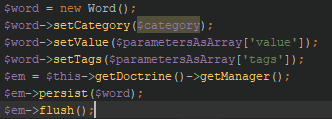
\includegraphics[width=150mm]{img/addWord.PNG}
        \caption{Création d'une nouvelle entrée dans la base de données}
        \label{Tux}
    \end{figure}

    \subsubsection{La lecture : Read}
    Pour la lecture, nous utilisons Doctrine, L'ORM de Symfony pour récupérer les données de la base et les renvoyer au client.

    \begin{figure}[h]
        \centering
        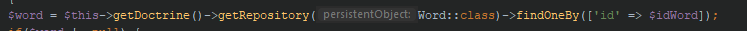
\includegraphics[width=150mm]{img/getWordById.PNG}
        \caption{Lecture des données de la base de données}
        \label{Tux}
    \end{figure}

    \subsubsection{La modification : Update}

    Pour modifier des données, on récupère (par la fonction de lecture) l'objet voulu grâce à son identifiant. On effectue ensuite les modifications directement sur l'objet grâce à des setters.
    Enfin on enregistre les données dans la base grâce aux méthodes persist(\$object) et flush().

    \subsubsection{La suppression : Delete}
    Pour la suppression, les données sont récupérées par lecture. Ensuite on utilise les méthodes de doctrine remove(\$object) et flush() pour enregistrer les changements.

    \begin{figure}[h]
        \centering
        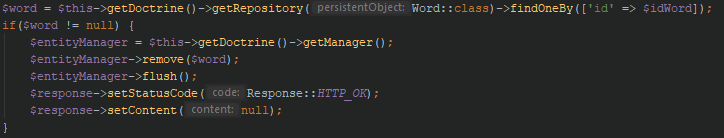
\includegraphics[width=150mm]{img/removeWord.PNG}
        \caption{Suppression d'une entrée dans la base de données}
        \label{Tux}
    \end{figure}

    \subsection{Implémentation de l'interpréteur}

    Afin de pouvoir générer les formes fléchies d'un mot, nous avons mis en place un algorithme d'interprétation des règles PFM.
    Voici une présentation du fonctionnement de l'algorithme

    \subsubsection{Récupération des données}
    Dans un premier temps, on se charge de récupérer les données nécessaires à la génération des formes fléchies.
    Les données nécessaires sont :
    \begin{itemize}
        \item Le mot
        \item Les tags du mots
        \item Les règles PFM de la même catégorie du mot
        \item Les associations de tags de la même catégorie du mot
    \end{itemize}
    \ref{PFM1}
    \smallbreak

    \begin{figure}[h]
        \centering
        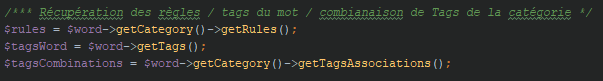
\includegraphics[width=150mm]{img/interpreteur_getData.PNG}
        \caption{Interpréteur PFM : Récupération des données utiles}
        \label{PFM1}
    \end{figure}

    \subsubsection{Premier filtrage des règles}

    La prochaine étape consiste à filtrer les règles afin de ne conserver que les règles dont les tags correspondent à ceux renseignés par le mot.\ref{PFM2}

    \begin{figure}[h]
        \centering
        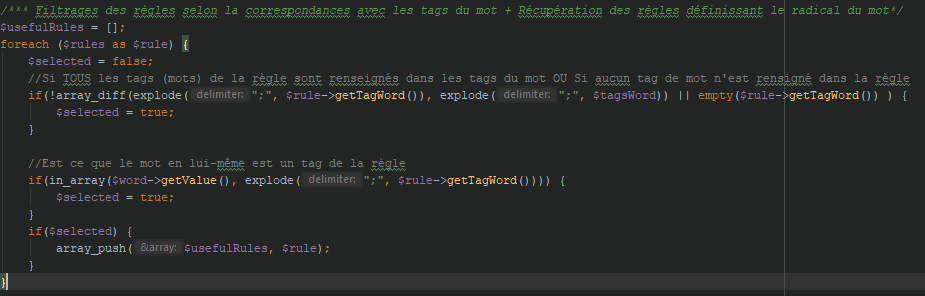
\includegraphics[width=150mm]{img/interpreteur_Filtrage1.PNG}
        \caption{Interpréteur PFM : Filtrage selon les tags du mot}
        \label{PFM2}
    \end{figure}


    \subsubsection{Début des traitements}
    A partir de cette étape, on parcoure toutes les combinaisons de tags enregistrés pour la catégorie du mot. Chaque combinaisons résultera sur une forme fléchie.

    \textbf{Second filtrage des règles} \\
    Pour chaque association de tags renseignés, on réitère l'étape de filtrage des règles en comparant les tags de la règle avec la combinaison de tags courante.
    A l'issue de cette étape, toutes les règles restantes sont compatibles pour générer une forme fléchie pour la combinaison de tags sélectionnée.\ref{PFM3}

    \begin{figure}[h]
        \centering
        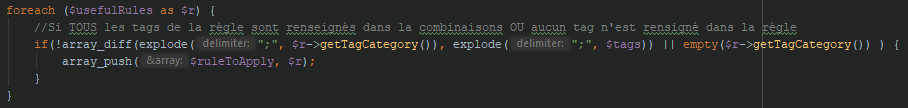
\includegraphics[width=150mm]{img/interpreteur_Filtrage2.PNG}
        \caption{Interpréteur PFM : Filtrage selon les combinaisons de tags}
        \label{PFM3}
    \end{figure}

    \textbf{Tri des règles par niveau d'application} \\
    Parmi les règles restantes, on les tries par niveau d'application pour faire une sélection de la règle à appliquer pour chaque niveau d'application.\ref{PFM4}

    \begin{figure}[h]
        \centering
        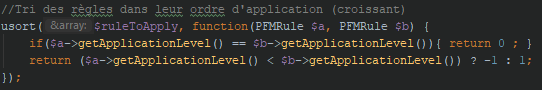
\includegraphics[width=150mm]{img/interpreteur_tri.PNG}
        \caption{Interpréteur PFM : Tri des règles par niveau d'application}
        \label{PFM4}
    \end{figure}

    \textbf{Sélection des règles à appliquer} \\
    Quand plusieurs règles ont le mêmes niveau d'application, on regarde laquelle est la plus spécifique pour la choisir.
    S'il existe 2 règles ou plus étant aussi spécifique l'une que l'autre, une exception est levée car aucun choix ne peut être fait.\ref{PFM5}

    \begin{figure}[h]
        \centering
        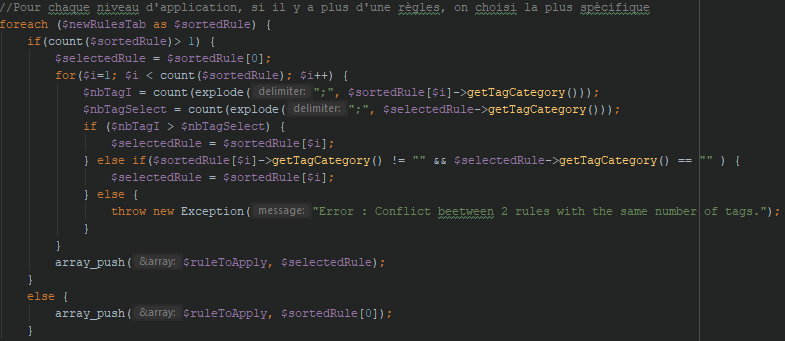
\includegraphics[width=150mm]{img/interpreteur_selection.PNG}
        \caption{Interpréteur PFM : Sélection de la règle la plus spécifique}
        \label{PFM5}
    \end{figure}

    \textbf{Application des règles} \\
    Enfin, chaque niveau d'application ne possède qu'une règle. Il suffit seulement de les appliquer dans l'ordre en remplaçant la chaîne \{word\} par le résultats des règles précédentes (en partant d'une chaîne vide à la base) et en y ajoutant les informations complémentaires. \ref{PFM6}

    \begin{figure}[h]
        \centering
        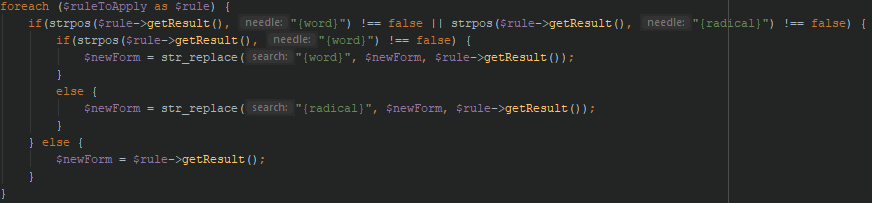
\includegraphics[width=150mm]{img/interpreteur_application.PNG}
        \caption{Interpréteur PFM : Application des règles}
        \label{PFM6}
    \end{figure}


    \subsection{Exporter le lexique}

    L'algorithme d'export\ref{Export} du lexique est très simple. En parcourant tous les mots de la base de données, on ajoute une ligne concernant le mot. Ensuite on cherche à générer les formes fléchies du mot et on ajoute une ligne dans le fichier pour chaque forme fléchie générée. \\
    Le fichier d'export respecte ainsi le format ci-contre :
    \begin{verbatim}
        <mot> <code-catégorie>["<categorie-name">] lemme="<mot>" {<mot-tags>}
        <forme-fléchie-générée> f["forme fléchie"] lemme="<mot>" {<tags-combinaison>}
        <forme-fléchie-générée> f["forme fléchie"] lemme="<mot>" {<tags-combinaison>}
        <mot> <code-catégorie>["<categorie-name">] lemme="<mot>" {<mot-tags>}
        <forme-fléchie-générée> f["forme fléchie"] lemme="<mot>" {<tags-combinaison>}
        <forme-fléchie-générée> f["forme fléchie"] lemme="<mot>" {<tags-combinaison>}
        ...
    \end{verbatim}
    Les tags sont séparés par des points-virgule.

    \begin{figure}[h]
        \centering
        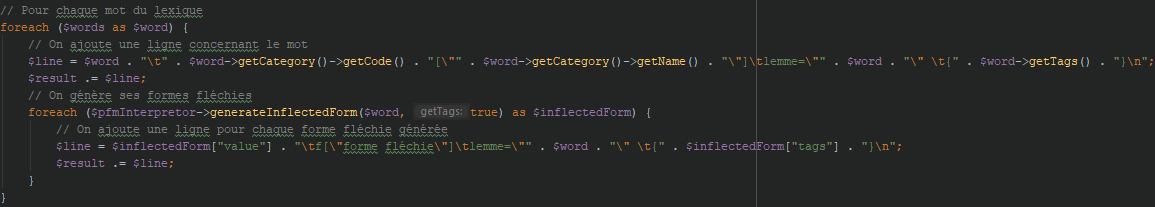
\includegraphics[width=150mm]{img/exportLexique.PNG}
        \caption{Export du lexique}
        \label{Export}
    \end{figure}

    \subsection{Importer le lexique}

    ON a ajouté une interface ou les utilisateurs peuvent importer les fichier sous format texte qui existent déjà. Pour cela on a définie 3 syntaxes différentes :
    \begin{itemize}
        \item La première correspond à celle respectée par notre fonctionnalité d'export.
        \item La deuxième correspond à la syntaxe du Lefff consultable le site de Lionel CLEMENT.
        \item Et La troisième correspond à la syntaxe du Lefff au format .mlex consultable sur le site de Benoît SAGOT..
    \end{itemize}

    \subsection{Les besoins non réalisés}

    A l'issue de ce projet, nous n'avons pas eu le temps d'implémenter certains besoins.
    En effet la gestion des utilisateurs avec des comptes utilisateurs et le système d'authentification n'a pas été mis en place. \\
    L'absence de cette fonctionnalité a engendré l'absence des rôles utilisateurs (visiteur, éditeur, éditeur expert et administrateur). Suite à cette absence, nous avons décidé d'autoriser l'accès à tous les utilisateurs à toutes les fonctionnalités implémentées. \\
    Le signalement de mot n'a pas été mis en place puisque tous les utilisateurs peuvent modifier ou supprimer les données d'un mot. \\
    Enfin la création d'un historique des modifications avec une possibilité d'inverser certaines modifications a aussi été mis de côté afin de privilégier le développement des fonctionnalités principales de l'application web.

    \subsection{Outils de développement}

    \subsubsection{Application web - Back-end et Interpréteur PFM}
    Pour la partie back-end de notre application le choix du langage de programmation s'est porté sur PHP\footnote{https://www.php.net/}.
    Ce langage, spécifique au développement web, est facile à prendre en main. De plus c'est un langage rapide avec beaucoup de fonctionnalités et de documentation.
    \smallbreak
    Nous avons ensuite choisi d'utiliser le framework Symfony\footnote{https://symfony.com/} dans la version 4.
    En effet ce framework intègre de nombreuses fonctionnalités permettant de répondre à certains des besoins identifiés précédemment :
    \begin{itemize}
        \item Doctrine, un ORM (Object Relational Mapping) permettant de manipuler les données de la base sous forme d'objet. En manipulant des objets, on évite les reqûetes SQL brutes, nous protégeant ainsi des injections SQL.
        \item Des fonctionnalités de sécurité contre les attaques XSS ou CSRF.
        \item Une architecture MVC (Modèle Vue Controleur) permettant ainsi de bien diviser notre code. En effet le entités sont implémentées séparément, et le contrôleur permet de traiter les actions.
        \item Une intégration facile de nouveaux services. L'interpréteur PFM ainsi que les méthodes d'import et d'export d'un lexique ont ainsi pu être ajoutées simplement.
        \item Une grande communauté et beaucoup de documentation permettant d'intégrer des packages existants à notre application pour simplifier le travail (exemple: afin d'éviter des problème de CORS (Cross-origin resource sharing) nous avons utilisé le package "NelmioCorsBundle"\footnote{https://github.com/nelmio/NelmioApiDocBundle} développé par "nelmio").

    \end{itemize}
    \smallbreak

    \subsubsection{Application web - Front-end}

    La partie front de l'application a été réalisé en Javascript avec le framework Angular 7\footnote{https://angular.io/}.
    Ce framework nous a permis de hiérarchiser notre code sous forme de composants réutilisable.
    L'utilisation de Typescript\footnote{https://www.typescriptlang.org/} par Angular a permis, de créer, de manière structurée, des modèle de données.
    Il permet aussi création de composants et de services à l'aide de commande à exécuter dans un terminal.
    Un système de gestion des routes permet d'appeler dynamiquement les composants sur la page sans avoir à régénérer le DOM (Pas de rafraîchissement de page à chaque changement d'url) permettant ainsi une navigation dynamique sur l'application.

    \subsubsection{Base de données}

    Pour le choix du Système de Gestion de Base de Données (SGBD), nous avons choisi MySQL\footnote{https://www.mysql.com/fr/} car il est très simple d'utilisation et il a été recommandé par le client.
    Ce SGBD s'intègre aussi facilement à notre framework Symfony permettant une configuration très simple.
    Niveau performance, ce choix est contestable lorsqu'il y un très grand nombre d'entrées. En effet la vitesse d'exécution des requêtes SQL en lecture ou en écriture est plus lente que d'autre SGBD comme PostgreSQL\footnote{https://www.postgresql.org/} par exemple.
    Ce choix est donc compréhensible au niveau facilité d'utilisation mais contestable au niveau des performances.

    \section{Analyse du fonctionnement et tests}

    Afin d'assurer le bon fonctionnement de notre application et d'être certains qu'elle répond bien aux besoins du client, des tests unitaires et des tests de performances ont été mis en place.

    \subsection{Test Unitaires - Front-end}

    Les tests de la partie front-end de l'application ont été réalisé par les outils Karma\footnote{https://karma-runner.github.io} et Jasmine\footnote{https://jasmine.github.io/}, tout deux intégré dans le framework Angular.
    Jasmine permet d'écrire des tests qui sont ensuite exécutés par Karma.
    Ce dernier peut être configuré afin de pouvoir visualiser les résultats des tests dans le navigateur. \\
    Les principaux tests concernent les composants. Ils permettent de vérifier que leur création a bien été réalisée et qu'ils ont bien été initialisés (via l'appel de la méthode ngOnInit()).
    Ensuite des tests interviennent pour vérifier que les composants ont été correctement générés sur la page web. \\
    Voici un exemple\ref{ListCategory} de tests du composant ListCategory permettant de tester si les catégories (\textbf{CATEGORIES}) sont bien initialisés par le service.
    Le test \textit{should set Categories correctly from service} vérifie si le nombre de catégorie est de 3 .
    \begin{verbatim}
        CATEGORIES = [
        {id: 1, code: 'adj', name: 'Adjectif'},
        {id: 2, code: 'v', name: 'Verbe'},
        {id: 3, code: 'nc', name: 'Nom Commun'}
        ];
    \end{verbatim}
    Enfin, le dernier test \textit{should create a tr for each category} permet de vérifier que le tableau html pour lister les catégories est bien créé.

    \begin{figure}[h]
        \centering
        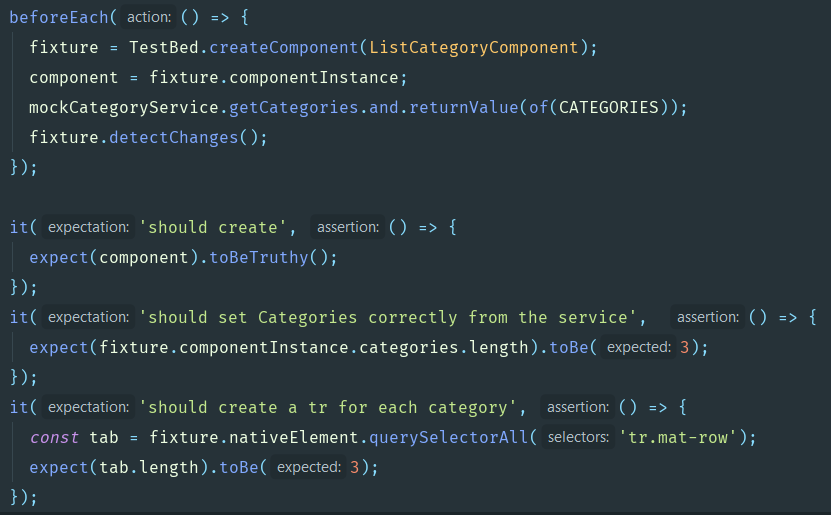
\includegraphics[width=170mm]{img/testlistcategory.PNG}
        \caption{Test Unitaire: Liste des catégories}
        \label{ListCategory}
    \end{figure}

    Pour tests des services nécessite d'envoyer des données à un serveur et de traiter la réponse.
    Pour simuler cette réponse, on utilise \textit{HttpTestingController}.
    Voici un exemple \ref{ServiceCombin} de tests d'un service : \newline
    \begin{figure}[h]
        \centering
        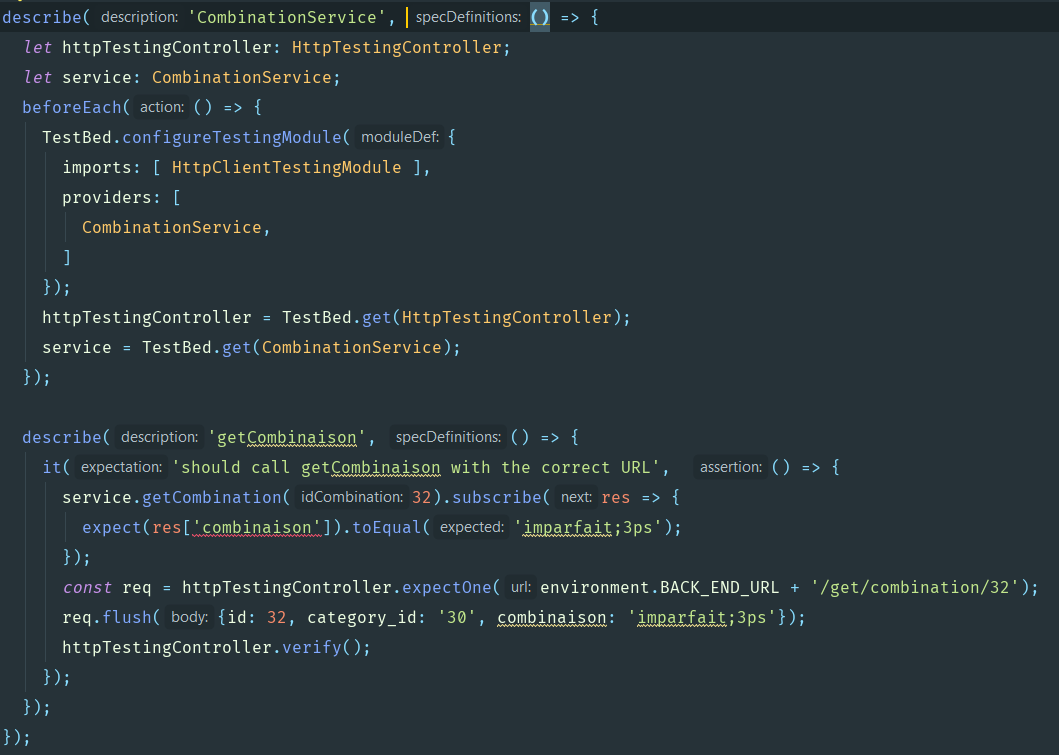
\includegraphics[width=170mm]{img/service Combinaison.PNG}
        \caption{Test Unitaire: Service des combinaisons}
        \label{ServiceCombin}
    \end{figure}

    Pour vérifier que notre méthode \textit{getCombinaison} de récupérer une combinaison, on appelle cette méthode avec un identifiant et on teste si la réponse attendue est la même que celle renvoyée par notre serveur simulé (  \textit{HttpTestingController}).
    La méthode \textit{exceptOne} permet de tester qu'une seule requête est envoyé.
    La méthode \textit{verify} de permet de vérifier la réponse. \newline

    \subsection{Test Unitaires - Back-end}

    Au niveau du back-end de l'application, les tests ont été réalisé à l'aide du framework de tests unitaire PHPUnit\footnote{https://phpunit.de/} et Guzzle\footnote{http://docs.guzzlephp.org/en/stable/} permettant de simuler un client pour notre application.
    Voici un exemple de tests permettant de vérifier le fonctionnement de l'ajout d'un mot :

    \begin{figure}[h]
        \centering
        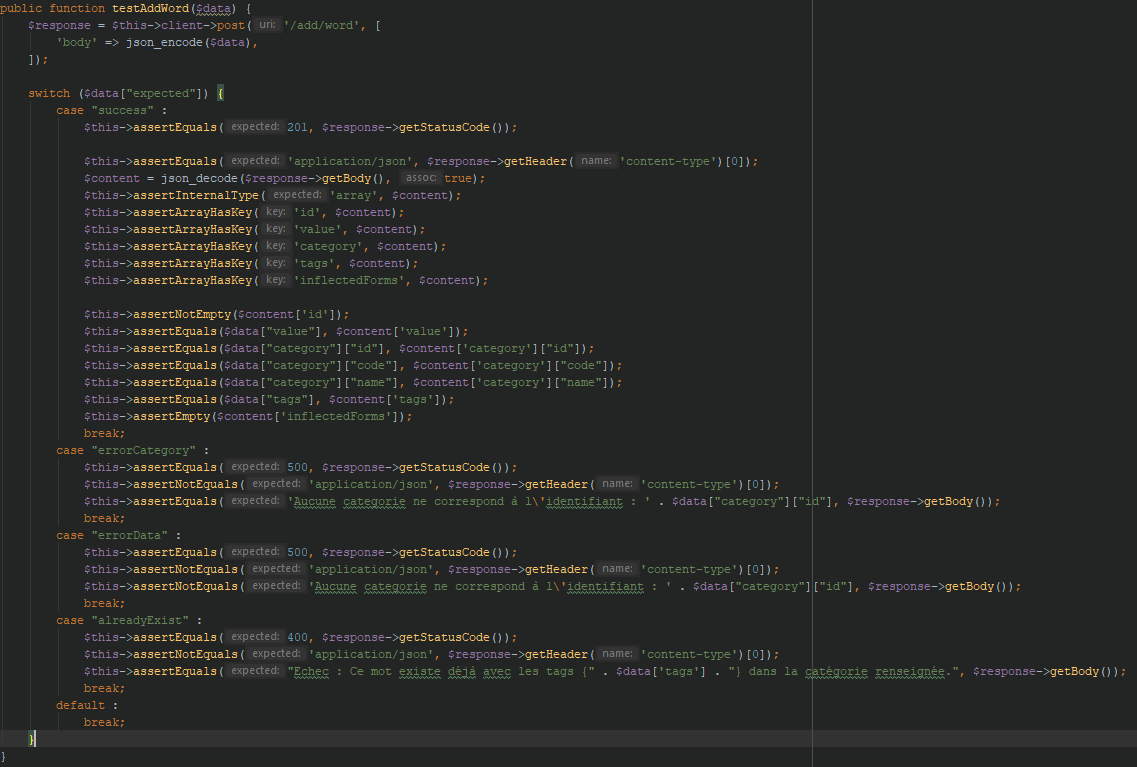
\includegraphics[width=170mm]{img/testaddWord.PNG}
        \caption{Test Unitaire: Ajouter un mot}
        \label{AddWordTest}
    \end{figure}

    Comme présenté sur la figure \ref{AddWordTest}, l'ajout de mot est effectué par des 4 ensembles de données :
    \begin{itemize}
        \item Un ensemble qui fonctionne
        \item Un ensemble possédant une catégorie inconnue
        \item Un ensemble avec des valeurs erronée
        \item Un ensemble avec des données existantes
    \end{itemize}

    On peut ainsi voir que tous les cas d'ajout sont testés. Selon les cas, le contenu de la réponse est testé.
    Le framework PHPUnit nous permet de tester le contenu de la réponse, son statut ainsi que toutes les en-têtes pouvant être renseignées.
    Par manque de temps, tous les tests n'ont pas pu être implémenter pour cette partie. Néanmoins ils devraient être similaires à ceux implémenter pour le controleur "WordController".

    \subsection{Tests de performances}

    Les tests de performances ont été réalisés manuellement. Ils nous ont permis de tester la rapidité des traitements, notamment pour l'import d'un lexique (action prenant actuellement le plus de temps quand l'import prend en compte un grand nombre de données).
    Le but de nos tests est de détecter si la lenteur du traitement de l'import est due à l'implémentation de nos algorithmes ou par les délais des requêtes SQL (sur lesquels nous n'avons pas de contrôle). \\
    Nous avons obtenus les résultats suivants (les temps obtenus sont des moyennes de plusieurs tests) : \\
    \textbf{En traitant l'import sans exécuter de requêtes SQL} \\
    \begin{itemize}
        \item Fichier de 500 lignes dont 499 enregistrements devraient être sauvegardés en base de données : 4.5 secondes
        \item Fichier de 1000 lignes dont 998 enregistrements devraient être sauvegardés en base de données : 6.4 secondes
        \item Fichier de 5000 lignes dont 4986 enregistrements devraient être sauvegardés en base de données : 21.8 secondes
        \item Fichier d'environ 550 000 lignes dont environ 120 000 enregistrements devraient être sauvegardés en base de données : 8.3 minutes
    \end{itemize}

    \textbf{En traitant l'import en exécutant les requêtes SQL} \\
    \begin{itemize}
        \item Fichier de 500 lignes dont 499 enregistrements devraient être sauvegardés en base de données : 13 secondes
        \item Fichier de 1000 lignes dont 998 enregistrements devraient être sauvegardés en base de données : 20 secondes
        \item Fichier de 5000 lignes dont 4986 enregistrements devraient être sauvegardés en base de données : 1.4 minutes
        \item Fichier d'environ 550 000 lignes dont environ 120 000 enregistrements devraient être sauvegardés en base de données : > 2h30
    \end{itemize}

    \smallbreak
    Ces temps ne prennent pas en compte la suppression des données de la base effectués avant l'import. Cette opération peut elle aussi prendre du temps lorsque la base contient un nombre important de données.

    \smallbreak

    Ces résultats nous ont montré que les problèmes de performances ne proviennent pas de nos algorithmes mais bien du très grand nombre de requêtes SQL a exécuter.
    Ces tests révèlent un inconvénient important dans le choix du système de gestion de base de données (SGBD) MySQL.
    Néanmoins, notre implémentation de l'application web ne limite pas son fonctionnement à ce SGBD, laissant ainsi la possibilité de changer facilement le SGBD.

    \newpage
    \section{Conclusion}
    \setlength{\parindent}{1cm}

    A l'issue de projet, nous avons fourni une application web répondant aux besoins principaux du client.
    En effet, malgré quelques besoins non implémentés, notre solution permet de d'importer un lexique dans une base de données et d'en consulter son contenu en en générant ses formes fléchies.

    \smallbreak

    \noindent En plus des besoins identifiés mais non implémentés, nous avons détecté des améliorations possibles à cette application :
    \begin{itemize}
        \item L'import et l'export d'un lexique pourrait prendre en charge les règles PFM et les combinaisons de tags.
        \item En cas de conflit entre 2 règles PFM de même niveau et étant aussi spécifique l'une que l'autre (situation censé être impossible mais aucun contrôle n'est effectué en base pour gérer cela) une erreur pourrait être renvoyée pour avertir l'utilisateur. Actuellement la première règle s'applique par défaut et peut donc générer une forme fléchie incohérente.
        \item L'utilisation d'un autre système de gestion de base de données pourrait permettre d'améliorer les performances (vitesse d'exécution) des fonctionnalités de génération des formes fléchies, d'import et d'export d'un lexique.
    \end{itemize}

    \smallbreak

    Pour conclure sur ce projet, nous avons eu du mal à comprendre le formalisme PFM et à trouver une manière de l'exploiter efficacement pour répondre à nos besoins. Ces incompréhensions nous ont fait perdre du temps dans l'implémentation de l'application. \\
    \noindent De plus, rendre notre solution générique à n'importe quel langage nous a demandé une conception longue et rigoureuse qui a provoqué de nombreux changements dans l'architecture de notre base de données. \\
    \noindent Néanmoins, ce projet nous a permis d'en apprendre beaucoup sur le formalisme PFM , la flexion des mots en général et de mettre en application nos compétences en programmation.

    \newpage
    \bibliographystyle{unsrt}
    \bibliography{references}

\end{document}